% This is a template for Ph.D. dissertations in the UCI format.
% 
% All fonts, including those for sub- and superscripts, must be 10
% points or larger.  Recommended sizes are 14-point for chapter
% headings, 12-point for the main body of text and figure/table
% titles, and 10-point for footnotes, sub- and super-scripts, and text
% in figures and tables.
%
% Notes: Add short title to figures, sections, via square brackets,
% e.g. \section[short]{long}.
%
\documentclass[12pt,fleqn]{ucithesis}

% A few common packages
\usepackage{amsmath}
\usepackage{amsthm}
\usepackage{array}
\usepackage{graphicx}
\usepackage{natbib}
\usepackage{relsize}

% Some other useful packages
\usepackage{caption}
\usepackage{subcaption}  % \begin{subfigure}...\end{subfigure} within figure
\usepackage{multirow}
\usepackage{tabularx}
\usepackage{siunitx}
\usepackage{amssymb}


% plainpages=false fixes the "duplicate ignored" error with page counters
% Set pdfborder to 0 0 0 to disable colored borders around PDF hyperlinks
\usepackage[plainpages=false,pdfborder={0 0 0}]{hyperref}



% Uncomment the following two lines to use the algorithm package,
% which provides an algorithm environment similar to figure and table
% ("\begin{algorithm}...\end{algorithm}"). A list of algorithms will
% automatically be added in the preliminary pages. Note that you
% probably want a package for the actual code to go with this (e.g.,
% algorithmic).
%\usepackage{algorithm}
%\renewcommand{\listalgorithmname}{\protect\centering\protect\Large LIST OF ALGORITHMS}

% Uncomment the following line to enable Unicode support. This will allow you
% to enter non-ASCII characters (such as accented characters) directly without
% having to use LaTeX's awkward escape syntax (e.g., \'{e})
% NOTE: You may have to install the ucs.sty package for this to work. See:
% http://www.unruh.de/DniQ/latex/unicode/
%\usepackage[utf8x]{inputenc}

% Uncomment the following to avoid "widowing", where page breaks cause
% single lines of paragraphs to float onto the next page (this is not
% a UCI requirement but more of an aesthetic choice).
%\widowpenalty=10000
%\clubpenalty=10000

% Modify or extend these at will.
\newtheorem{theorem}{\textsc{Theorem}}[chapter]
\newtheorem{definition}{\textsc{Definition}}[chapter]
\newtheorem{example}{\textsc{Example}}[chapter]

% Matrix
\newcommand{\matr}[1]{\mathbf{#1}}


% Macros for title, author, abstract, etc.
\thesistitle{Applications of Synthetic Microchannel and Nanopore systems}

\degreename{Doctor of Philosophy}

% Use the wording given in the official list of degrees awarded by UCI:
% http://www.rgs.uci.edu/grad/academic/degrees_offered.htm
\degreefield{Physics}

% Your name as it appears on official UCI records.
\authorname{Preston Hinkle}

% Use the full name of each committee member.
\committeechair{Dr. Zuzanna S. Siwy}
\othercommitteemembers
{
  Dr. Jun Allard \\
  Dr. Ilya Krivorotov
}

\degreeyear{2017}

\copyrightdeclaration
{
  {\copyright} {\Degreeyear} \Authorname
}

% If you have previously published parts of your manuscript, you must list the
% copyright holders; see Section 3.2 of the UCI Thesis and Dissertation Manual.
% Otherwise, this section may be omitted.
% \prepublishedcopyrightdeclaration
% {
% 	Chapter 4 {\copyright} 2003 Springer-Verlag \\
% 	Portion of Chapter 5 {\copyright} 1999 John Wiley \& Sons, Inc. \\
% 	All other materials {\copyright} {\Degreeyear} \Authorname
% }

% The dedication page is optional.
\dedications
{
	
}

\acknowledgments
{
	
}


% Some custom commands for your list of publications and software.
\newcommand{\mypubentry}[3]{
  \begin{tabular*}{1\textwidth}{@{\extracolsep{\fill}}p{4.5in}r}
    \textbf{#1} & \textbf{#2} \\ 
    \multicolumn{2}{@{\extracolsep{\fill}}p{.95\textwidth}}{#3}\vspace{6pt} \\
  \end{tabular*}
}
\newcommand{\mysoftentry}[3]{
  \begin{tabular*}{1\textwidth}{@{\extracolsep{\fill}}lr}
    \textbf{#1} & \url{#2} \\
    \multicolumn{2}{@{\extracolsep{\fill}}p{.95\textwidth}}
    {\emph{#3}}\vspace{-6pt} \\
  \end{tabular*}
}

% Include, at minimum, a listing of your degrees and educational
% achievements with dates and the school where the degrees were
% earned. This should include the degree currently being
% attained. Other than that it's mostly up to you what to include here
% and how to format it, below is just an example.
\curriculumvitae
{

\textbf{EDUCATION}
  
  \begin{tabular*}{1\textwidth}{@{\extracolsep{\fill}}lr}
    \textbf{Doctor of Philosophy in Physics} & \textbf{2017} \\
    \vspace{6pt}
    University of California, Irvine & \emph{Irvine, California} \\
    \textbf{Bachelor of Science in Physics} & \textbf{2011} \\
    \vspace{6pt}
    The Ohio State University & \emph{Columbus, Ohio} \\
  \end{tabular*}

\vspace{12pt}
\textbf{RESEARCH EXPERIENCE}

  \begin{tabular*}{1\textwidth}{@{\extracolsep{\fill}}lr}
    \textbf{Graduate Student Researcher} & \textbf{2012--2017} \\
    \vspace{6pt}
    University of California, Irvine & \emph{Irvine, California} \\
  \end{tabular*}

\vspace{12pt}
\textbf{TEACHING EXPERIENCE}

  \begin{tabular*}{1\textwidth}{@{\extracolsep{\fill}}lr}
    \textbf{Teaching Assistant} & \textbf{2012--2016} \\
    \vspace{6pt}
    University of California, Irvine & \emph{Irvine, California} \\
  \end{tabular*}
  
   \begin{tabular*}{1\textwidth}{@{\extracolsep{\fill}}lr}
    \textbf{Teaching Assistant} & \textbf{2012} \\
    \vspace{6pt}
    The Ohio State University & \emph{Columbus, Ohio} \\
  \end{tabular*}


  
\pagebreak

\textbf{REFEREED JOURNAL PUBLICATIONS}

	\bibentry{Hinkle2017}
	\bibentry{Yang2016}
	\bibentry{Qiu2015}

% \vspace{12pt}
% \textbf{REFEREED CONFERENCE PUBLICATIONS}
% 
% 	\mypubentry{Awesome paper}{Jun 2011}{Conference name}
% 	\mypubentry{Another awesome paper}{Aug 2012}{Conference name}

\vspace{12pt}
\textbf{SOFTWARE}

  \mysoftentry{nanoIV}{https://github.com/tphinkle/nanoIV}
  {Keithley 6487 Picoammeter control GUI program. Allows measurement of current-voltage and time-series data.}
  
  \mysoftentry{pore stats}{https://github.com/tphinkle/pore_stats}
  {GUI program and Python library for extracting and analyzing resistive pulse data.}
  
  
}

% The abstract should not be over 350 words, although that's
% supposedly somewhat of a soft constraint.
\thesisabstract
{
	There are a diverse range of applications involving fluidic systems at the micro- and nanoscale. Making use of the nanoscale physics that takes place in the vicinity of charged surfaces, there is the possibility that nanopores, holes on the order of $\SI{1}{nm}$ in size, could be used to make complex integrated ionic circuits. For inspiration on what such circuits could achieve we only need to look to biology systems, immensely complex machines that at their most basic level require precise control of ions and intercellular electric potentials to function. In order to contribute to the ever expanding field of nanopore technology, we engineered novel hybrid insulator-conductor nanopores that behave analagously to ionic diodes, which allow passage of current flow in one direction but severely limit the current in the opposite direction. Not only did the behavior of the pore give key insights into the fundamental physics and chemistry underlying the electrical double layer, but it can also be considered as a standard rectifying element in ionic circuits. Another application of ion conducting channels is a particle sensing method, known as resistive pulse sensing. We present three main experiments that expand the capacity of resistive pulse sensing applications. First, we demonstrate how resistive pulse sensing in pores with longitudinal irregularities can be used to measure the lengths of individual nanoparticles. Then, we describe an entirely new hyridized method, whereby resistive pulse sensing is combined with optical imaging. The hybrid method allows for validation of the resistive pulse signals, and will greatly contribute to their interpretability. We present experiments that explore some of the possibilities of the hybrid method. Then, building off the hybrid method we present our findings for experiments performed with using resistive pulse sensing to measure the deformability of particles. Using a novel microfluidic channel design, we were able to reproducibily induce deformation of cells in a controlled manner. We describe how these deformations could be detected with the resistive pulse signal, paving the way for resistive pulse sensing based cell deformability cytometers.
}


%%% Local Variables: ***
%%% mode: latex ***
%%% TeX-master: "thesis.tex" ***
%%% End: ***


% Add PDF document info fields
\hypersetup{
	pdftitle={\Thesistitle},
	pdfauthor={\Authorname},
	pdfsubject={\Degreefield},
}


%\theoremstyle{definition}
%\newtheorem{definition}{Definition}[section]
 
%\theoremstyle{remark}
%\newtheorem*{remark}{Remark}

% Uncomment the following to have numbered subsubsections (by default
% numbering goes only to subsections).
%\setcounter{secnumdepth}{4}


% Set this to only select a subset of the includes directives below.
% Very handy to speed up compilation if you're working on a certain
% part of your thesis. It conserves page numbers, references, etc.
% even for non-included files.
%\includeonly{chapter1}

\begin{document}

% Preliminary pages are always loaded (TOC, CV, etc.)
\preliminarypages

% Include the different components of your thesis, in separate files.
% Using \include allows you to set \includeonly above.
\graphicspath{{../images/ch1/}}	% Image directory


\chapter{Introduction}

	The introduction to this dissertation is structured as follows. First, we introduce the main topic of this dissertation and of my PhD research work, the nanopore. This section serves to introduce the reader first, to the basic definition of a nanopore and then to some of their applications, in addition to miscellaneous facts about nanopores that provide context for why they are of interest to scientists. This section is entirely qualitative and does not aim to make any statements about the underlying physics needed to understand nanopore systems. Subsequently, I introduce in three stages the physics that is relevant to nanopore systems. It turns out that if we take a macroscaled system (say, a tube rather than a nanotube) and slowly shrink it in size, then as the system size shrinks new types of physics emerges and become increasingly relevant to the system. We will start by addressing the relevant physics at the milliscale and shrink in intervals of powers of three, stopping at the sub-nanoscale. Therefore, the progression looks like milli-, micro-, nano-, and finally, sub-nano-. To provide a bigger picture of the journey through different length scales, the progression looks like ant, cell, protein, molecule.

	\section{Nanopores}

		Unlike most physics jargon, the name nanopore is entirely self-explanatory. In fact, the following is a terse (but accurate) definition of a nanopore:


		\begin{definition} \label{def:nanopore}
			A nanopore is a hole on the order of $\SI{1}{nm}$ in size
		\end{definition}


		As we will discover, this definition, while accurate, does not do justice to the field of nanopore research. 

		Nanopores generally belong to two classes, biological and synthetic. Because nanopores can be found in biology, many scientists are interested in studying them in their own right, to better understand how biological systems function. On the other hand, nanopores, both biological and synthetic, can be used in a surprisingly large variety of applications, with the total count of such applications constantly increasing. In this section we will briefly discuss the types of biological nanopores and where they are found in nature, and then move on to describing different types of synthetic nanopores. Given the loose criteria required by \ref{def:nanopore} for something to constitute a nanopore, listing off every type of either biological or synthetic nanopores would be impossible; instead, I seek to introduce the most relevant types, with an admitted bias towards the types of nanopores I am most familiar with and that I have worked with in my research. After discussing the various types of nanopores, I will give a summary of applications in which nanopores see use. Some of these applications, for instance resistive-pulse sensing, are a major part of this dissertation and will therefore be discussed in much greater detail later on, while others, such as DNA sequencing, are important enough to be mentioned but not discussed in significant detail later on. An extensive list of references, including those not explicitly referenced in this work, will be included should the reader wish to read more on a particular topic.

		\begin{figure}[h]
			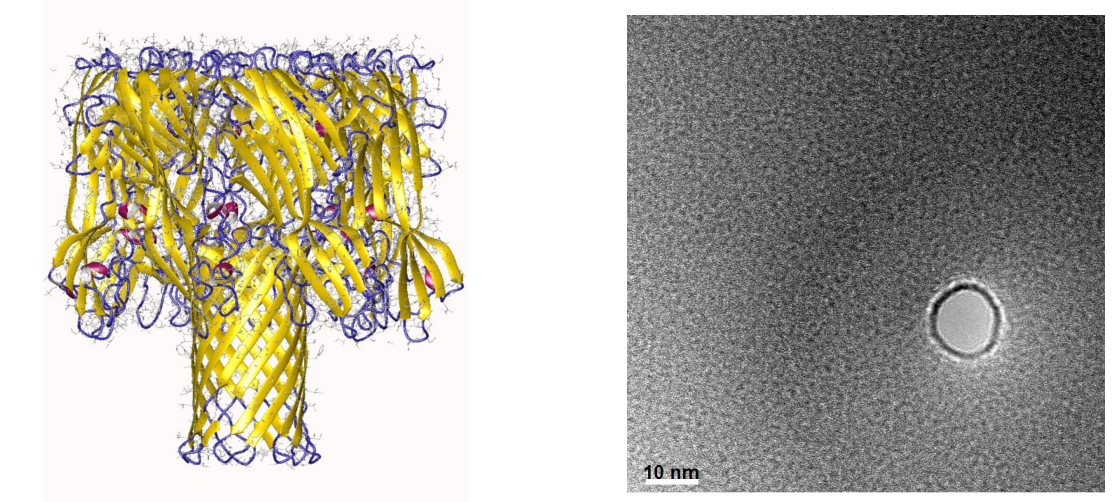
\includegraphics[width=\textwidth]{bio_synth_nanopores.png}
			\caption{Two types of nanopores. \textbf{Left:} Alpha-hemolysin, a biological type of nanopore approximately $\SI{1}{nm}$ in diameter. \textbf{Right:} A silicon nitride nanopore drilled using a transmission electron microscope (TEM), approximately $\SI{10}{nm}$ in diameter.}
		\end{figure}

		\subsection{Biological nanopores}

			As mentioned before, nanopores exist naturally in biology. Their most important function is to enable passage from one region to another, much like a tunnel does; however, where a tunnel permits cars, trucks, etc., the passengers in nanopore systems are water, ions, proteins, etc. Nanopores typically connect regions that are necessarily divided in order for a cell to function. Membrane-bound nanopores are structures made out of protein that are embedded in a cell's lipid bilayer that connect the outside of a cell to the inside of a cell. They serve the useful function of regulation osmotic pressure by allowing water to enter and exit the cell, and also balance voltage differences by allowing passage of important electrolytes such as sodium, potassium, and chloride. Therefore, maintaining homeostasis is one of the chief functions of these types of nanopores. These pores also enable passage of messenger molecules that enable extracellular messenging, crucial to all multicelled organisms. Like lipid bilayer pores, there are also pores in the nuclear membrane that enable transport into and out of the nucleus of a cell. These pores' chief responsibility is to allow the passage of messenger molecules in and out of the nucleus. 

			The most fascinating property of nanopores is their capacity for active management of transport. For instance, some nanopores may open or close when the voltage difference across them surpasses a threshold; other types of nanopores are \textit{ion selective}, permitting passage of some types of ions while denying passage to others. \textit{Active} transport is absolutely crucial to biological systems; if all nanopores were passive holes that permitted anything to pass through, the system would equilibrate in a homogeneous, non-functional soup of maximum entropy---life simply could not exist. Fortunately for us, nanopores are active transport regulators and life goes on. Going back to our tunnel analogy, nanopores act more like regulated tunnels, for instance some with guards that permit small cars only and deny trucks, or permit passage in only one direction, etc.

		\subsection{Synthetic nanopores}

			Advances in nano- and microfabrication have led to an enormous number of different types of synthetic nanopores. Synthetic nanopores can be made from a variety of different types of materials, and often their geometry (shape and size), as well as their surface chemistry properties, can be tailored to introduce specific types of behavior. However, the type of material used to make the nanopore most often determines the types of geometries and chemistries that are allowed. The following is a list of common types of nanopores, with a description of the type of material they are made from, their permissable length scales, and other miscellaneous relevant facts about them.

			\textbf{Monolayer pores.} The invention of graphene, a monolayer of carbon atoms, and later MoS2, opened the possibility of creating nanopores with a length of a single atom. These types of pores are created by punching through the thin monolayer, typically with an electron or ion beam. While still a very new field of study, these pores may see future use in desalination (removing electrolyte ions from water).

			\textbf{Carbon nanotubes.} A carbon nanotube can be conceptually understood as a rolled up tube of one or a stack of graphene layers. Graphene is a a monolayer of carbon atoms, and therefore a carbon nanotube itself is a type of pure crystal structure. The lattice arrangement of carbon atoms permits only certain tube diameters, which itself depends on the chirality of the tube (the way the tube is rolled up). Carbon nanotubes are interesting to researchers because of the exotic behaviors they exhibit that are not present in most other types of nanopores---for instance, they exhibit frictionless transport of water, hydrogen-dominant conductance (\textit{via} the Grotthus mechanism), ion selectivity, and more. As of the submission of this dissertation, the use of CNTs as nanopore is still a new field of study, and the physical mechanism for the previously mentioned behaviors is still poorly understood. Nevertheless, the extreme confinement ($\SI{1}{nm}$ and below for small CNTs) and the atomic-level precision of their structure are believed to be responsible. Another interesting aspect of the smallest CNTs is the breakdown of mean-field physics in describing their behavior. For instance, the Navier-Stokes equations which describe fluid dynamics, breaks down at this level because the water must be considered at the molecular level; the mean-field approach is no longer valid. Because they are still new, we do not yet know the exact applications that these nanopores will see use in. However, it is likely that they could be used in desalination applications (removing ions from water), or in ionic circuits as cation selective elements.

			\textbf{Silicon nitride.} Silicon nitride is a type of crystalline semiconductor that permits engineering of nanopores through several different fabrication processes. Briefly, very thin layers of silicon nitride (e.g.~$10-100$ nm) are grown, and a hole is bored through via either electron or ion beam milling. For instance, in one project of this dissertation I describe a project conducted with silicon nitride pores that were drilled via high-energy transmission electron microscope (TEM). Depending on the type of mill used (ion or electron), the size of these nanopores ranges, but the diameter is generally in the range of $1-100$ nm. One advantage of silicon nitride pores is their smooth interior geometries, as well as the native silane chemistry on the surface that permits many types of chemical modifications. These types of pores are used as ionic rectifiers (after modification), and in resistive pulse applications.

			\textbf{Glass nanopipettes.} Quartz pipettes can be heated and slowly stretched, reducing the tip diameter with the possibility of reaching the nanoscale. Unlike the previously mentioned pores which all had an approximately cylindrical geometry, these nanopipettes have a conical shape. These pores have a couple advantages. First, the stretching process itself is simple and can be used to create many pores over a short amount of time. Second, the surface chemistry of the glass or quartz is amenable towards chemical modification. These pores may be used in ionic circuits, in resistive pulse sensing, or as a surface probe, by monitoring the current through the pipette as it approaches a charged surface.

			\textbf{Track-etched polymer nanopores.} These types of pores are perhaps the most robust, dependable types of nanopores. Pore formation is a multistep process. First, untouched polymer membranes are irradiated by a single heavy isotope of an element such as gold and xenon, that has been accelerated to high speeds in a particle accelerator. The ion rips through the membrane, uniformly dispersing some of its kinetic energy into the surrounding polymer, and breaking the bonds in the polymer surrounding its trajectory. This location of damaged polymer bonds is known as the `damage track'. An ion detector is placed at the exit point of the membranes so that the beam can be switched off when a single ion is detected. This detection, along with a solid mask placed in front of the beam that blocks the vast majority of the ions in the beam, ensures that films that only have a single damage track can be prepared. This step, known as irradiation, must be performed off-site at a particle accelerator. After heavy ion irradiation, the membranes are immersed in an etchant solution such as NaOH or KOH. The etchant preferentially attacks the polymer in the damage track, clearing out the polymers along the track much faster than elsewhere in the membrane. Once the track has been etched out, the rest of the membrane is isotropically etched slowly by the NaOH. Pores prepared by the track-etch technique have a few advantages, including a customizable size and geometry. By putting etching solution on only one side of the membrane, it is possible to create conical pores of various aspect ratios. By applying a voltage across the pore during the etching process, the ionic current can be monitored and the etching process can be stopped at a particular current level, allowing the researcher customize the pore diameter. Another advantage of these pores is the carboxyl groups native to their surfaces, which permit many types of useful chemical modifications.

			\textbf{Hybrid biological-synthetic nanopores.} Biological nanopores, such as alpha hemolysin, aerolysin, or MSPA to name a few, can be isolated from their host biological systems and inserted into synthetic systems, forming a hybrid biological-synthetic complex. In these cases, the pore is entirely biological, but the complex does not appear naturally in nature, and the pores may be used in engineering or scientific applications. To make matters even more confusing, such pores may also be genetically modified to change some of their behavior, meaning they are derived from biology but are synthesized in the lab. For instance, the company Oxford nanopore invented a genetically modified alpha hemolysin nanopore that is especially adept at differentiating between nucleotides, and is currently being used in DNA sequencing applications.

		\subsection{Applications (introductions)}

			So far, I have hinted at or referred to nanopore applications without getting into specifics. Just as there are too many types of nanopores to enumerate, there are too many applications of nanopores to list them all off. This is a list of some of the most important applications of nanopores.

			\textbf{Analyte detection and characterization with the resistive pulse technique.} Surprisingly, nanopores may be used as a sort of particle characterizer using something called the resistive pulse technique, which works as follows. A voltage is applied across the nanopore, which induces a measurable ionic current to flow through the channel. If a particle enters the nanopore, the particle will occupy a volume that otherwise would be occupied by high-conductivity ions, increasing the pore's resistance, and decreasing the measured current. It turns out that by studying the nature of the decrease in the current, we can gather some information about the transiting particle. For instance, by counting the number of pulses in the measured ionic current, we can determine the concentration of particles in the suspension. The size of the particle can be determined by relating it to the depth of the pulse---larger particles block the current to a larger degree, and therefore create deeper resistive pulses. If the particle is at least partially driven through the channel \textit{via} electrophoresis (discussed later), then the particle's surface charge can be determined by the length of the pulse, or `dwell time' of the particle.

			One advantage of resistive pulse sensing is its scale-independence, which is a result of the generality of the physics involved. For this reason, resistive pulse sensing has been used in a large number of applications. The original use of the resistive pulse technique was in performing red blood cell counts (channel size approximately $\sim\SI{100}{\mu m}$ which was achieved by Coulter in 1953; this is the reason why sometimes the resistive pulse technique is referred to as the Coulter counter priniciple, or simply the Coulter principle. Since Coulter's original design, the resistive pulse technique has been used in counting smaller specimens such as exosomes, proteins, and viruses, used to measure particle rigidity, and perhaps most importantly, in DNA sequencing. The basic idea of resistive-pulse sensing for DNA sequencing is that the four types of nucleotides have slightly different sizes, and therefore lead to four unique current blockages. DNA can be slowly threaded through a nanopore while the current is monitored, and the discrete states in the resulting time-series of the measured current yield the sequence of DNA.

			\textbf{Water desalination.} Charged nanopores are slightly ion selective, meaning they preferentially allow one polarity of charge over another to pass through. If one side of a nanopore membrane is filled with electrolyte solution and a pressure is applied, water will pass through the pore, and due to the selectivity of the membrane, fewer ions will pass through than are contained in the bulk. In this way, nanopores can be used for water desalination. This mechanism of salt rejection is electrostatic, since the finite potential in the vicinity of the pore walls is responsible for screening ions. Traditional water desalination relies on reverse osmosis membranes that are completely impermeable to salts, and therefore \textit{sterically} reject ions.  In future sections we will discuss the physics involved with water desalination.

			\textbf{Nanopore ionics and ionic circuits.} Ion transport is fundamentally important to all cellular life. At the most basic level, single cells maintain homeostasis with their environment by maintaining a careful balance of salt ions across their membranes. This balance is regulated by a rich variety of ion channels, each with their own specific functionality. For instance, potassium can diffuse through potassium channels at nearly the bulk diffusion rate (i.e. the channel hardly impedes their motion), while sodium is completely blocked, an amazing feat considering the ions are nearly identical, save a minute difference in their hydration radii. Beyond maintaining homeostasis, ion channels are also responsible for propagating electric signals along axons, crucial for signaling in multicellular organisms. 

			One of the holy grails in nanopores is being able to reproduce the functionality of these biological pores, that were created by millions or billions of years of evolution, in synthetic systems. The ability to do so could create a revolution in ion conducting systems, analagous to the revolution in electronics that was created by the invention of the solid-state transistor. However, the goal of ionics is not to replace wires, capacitors, and transistors with ion channels and pores; indeed, ions travel orders of magnitude slower than electrons, and therefore ionic systems are expected to act more slowly than electronic systems. Instead, integrated ionic circuits could be used for complex signaling since each ion carries its own information, and for controlling the transport of biomolecules. One needs only to look at biology for inspiration on the application of complex ion channels.

	\section{Nanopore science---physics and chemistry}

		The actors at play in nanopore systems include the fluid solvent that fills the pore and its exterior regions, the charged ion species, the pore surfaces themselves, the electrodes, and finally, any particles (cells, biomolecules, etc.) present in the system. In the following sections we will delve into the physics that determines the interplay between these actors. As it turns out, as we shrink a system size from the macro to nanoscale, new regimes of physics become increasingly important. Therefore, not all of the physics mentioned in the upcoming sections are applicable to all length scales; for instance, the properties that make nanopores behave more interesting than just an open space only emerge close to the nanoscale, and are irrelevant in microscale systems. We can think of four distinct length scales at which the physics, and hence the system behavior, is sufficiently differentiated so as to give that scale its own identity. These scales are the milliscale, microscale, nanoscale, and subnanoscale. For example, microscale physics is sufficiently different from nanoscale physics that one may be an expert in one of hte two, but not the other. While the actors at play in these two systems---water, ions, particles, etc.---are all the same, the observed behavior of the systems can still be quite different. To give a brief preview of what is to come, the most important physics involved in nanopore theory is fluid mechanics (to describe the forces on the solvent), electrostatics (because of the voltage boundary conditions imposed by electrodes and charged surfaces), electrokinetics (due to migration of charged species under electric fields), and statistical mechanics (to describe the ensemble behavior of the ions and diffusion). Before moving on, it is important to note that concepts in chemistry are also very important in nanopores. For instance, electrochemical theory explains the mechanism for how an ion current turns into an electron current at the electrode-liquid interface. As another example, the charges present at the surfaces in almost all surfaces in contact with a fluid are due to the chemical groups, and their charged state. In the following sections, whenever chemistry is relevant, I will mention its role in creating the entity that we then go on to describe insofar as is possible with physics alone. For example, I will acknowledge the charge of a nanopore is due to chemical groups attached to its surface, but will then proceed agnostically, treating the charges as if they were a perfect model surface-charge, uniformly distributed over the surface of the pore. Chemistry will be invoked in the main chapters of this thesis as it relates to specific aspects of the projects.

		\begin{figure}[h]
			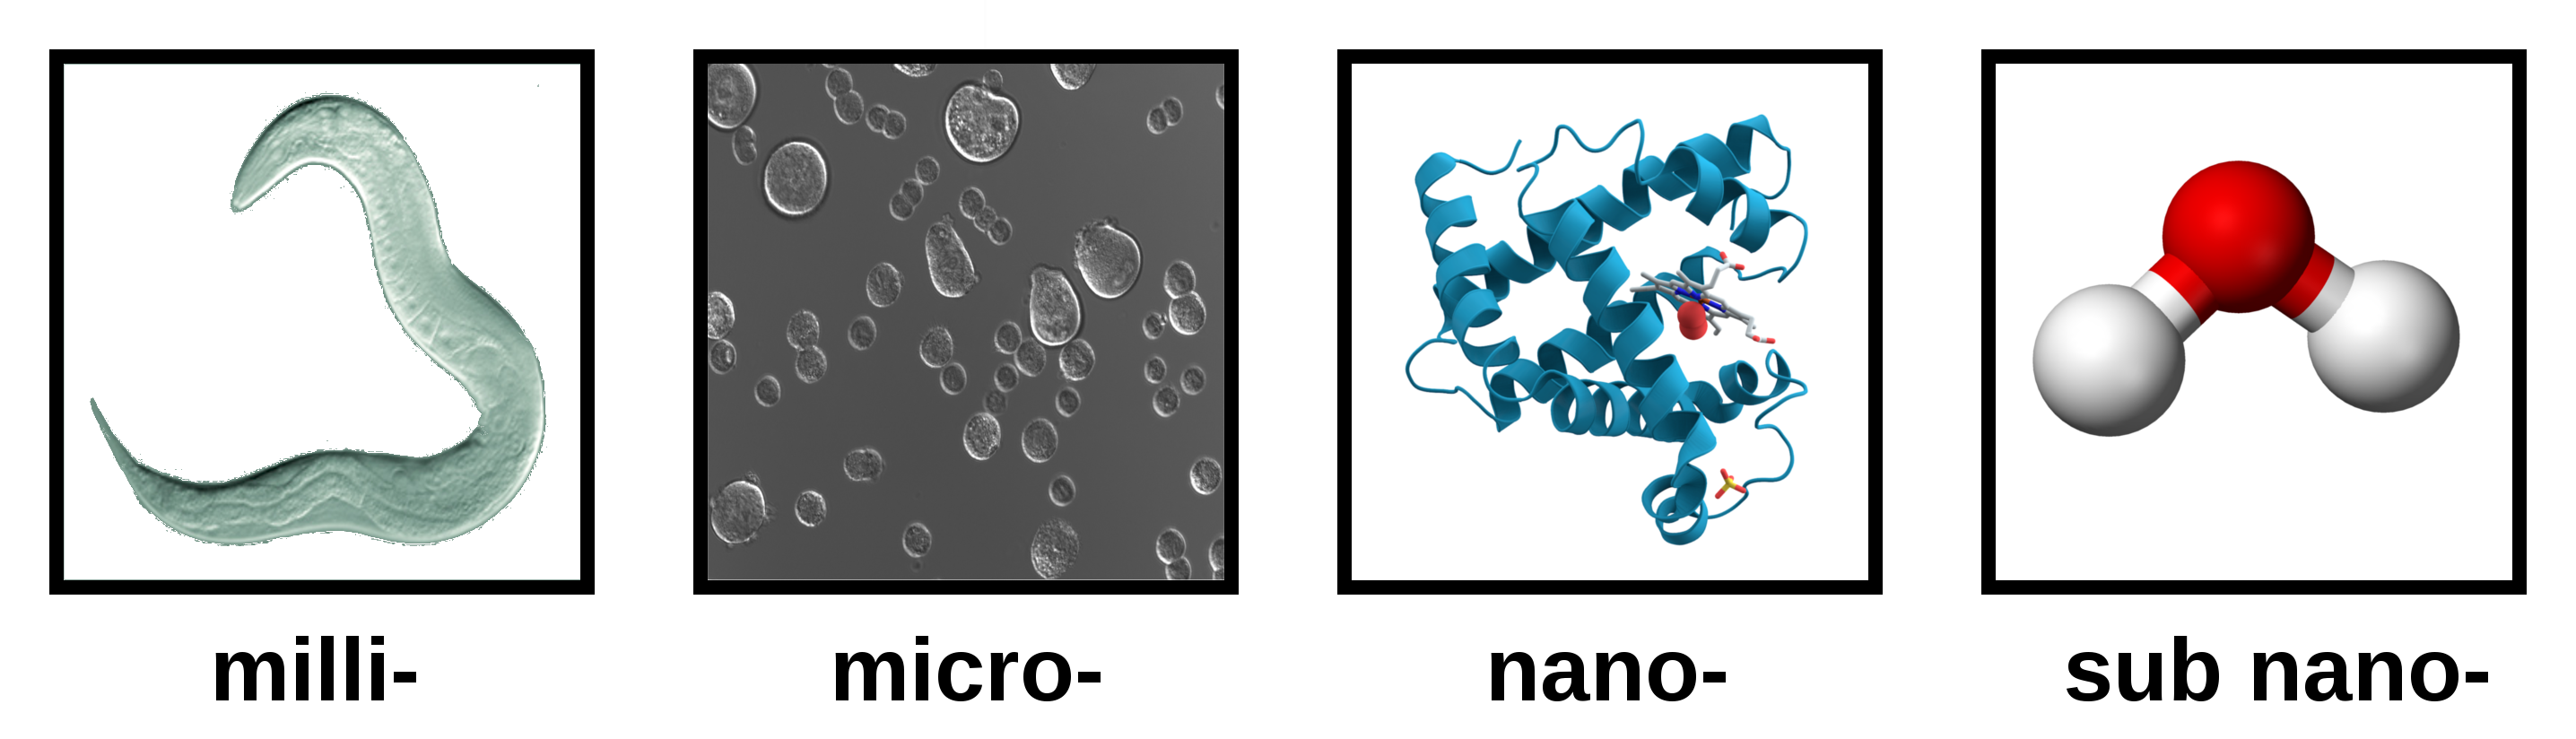
\includegraphics[width=\textwidth]{scales.png}
			\caption{Four important length scales for fluidics and surface forces. \textbf{milli-}: Caenorhabditis elegans (\textit{c. elegans}) sample, approximately 1 mm in length. Surface tension and capillary forces become significant at this length scale. Fluid dynamics is described by the complete Navier-Stokes equations. \textbf{micro-}: HCT-116 (colorectal cancer) cells, approximately $\SI{10}{\mu m}$ in diameter. Surface effects become increasingly important. Gravity becomes increasingly negligible, and systems under small applied pressures are described by having low-Reynolds number. \textbf{nano-}: A protein. Fluidic systems are dominated by surface forces. Liquid within $\SI{1}{nm}$ of surfaces is entirely contained within the electrical double layer. Fluid is completely non-inertial. \textbf{sub nano-}: A water molecule. Mean-field approximations are no longer valid. Navier-Stokes breaks down. Physics is determined entirely by electrostatic and Van der Waals forces between individual atoms and molecules.}
		\end{figure}
		
		\subsection{Pore/channel}
		
			The pore/channel itself is the primary actor of interest in our systems. The pore is created in some material, and the material properties as well as the fabrication procedure dictate the shape and geometry of the pore. As we will see, ionized chemical groups on the surface of the pore play as important a role as geometry in determining the behavior of the pore system.
		
		\subsection{Electrolyte solutions}
		
			Life on Earth exists in primary a \textit{fluid} environment, with the primary fluid being water. Water is the solvent for the chemistry of our bodies, and acts as the medium that allows electrolytes to ionize and transport between areas. In synthetic nanopore systems, we immerse our pore in an electrolyte solution that fills the channel, and under an applied voltage induces conduction of ions.
			
		\subsection{Electrodes}
		
			In order to create an external voltage in our system, an electronic voltage must be transformed into an ionic voltage potential. This is achieved \textit{via} ion electrodes, which allow transferrance of electrons into the ions of the solution and vice-versa, and the ions from the electrode then become the conductors in the system. This transferrance is known as a redox reaction in chemistry. For the rest of the thesis, unless specified we turn a blind eye to the chemical conversion process at the surface of the electrodes, and pretend that our electrodes are ideal voltage sources.
			
		\subsection{Particles}
		
			Because so many of the applications of interest for nanopore and microchannel studies involve biomolecule manipulation, we often work with electrolyte solutions that contain a suspension of particles in addition to the ions. The particles used are tied to the application, but often respond in the same way to forces present in teh system.

		\subsection{Equations of motion for fluidic systems---Navier--Stokes equations}
		
			One of the major actors in nanopores systems is the fluid solvent, which may remain at rest or, more commonly, move in response to forces present in the system. Because the motion of the solvent couples to the motion of other actors present in the system, understanding the physical laws governing the fluid medium is crucial. For systems large compared to the size of molecules, we make the approximation that the fluid is a continuous rather than discrete medium. In reality, we know that fluids are not continuous but ar emade up of discrete atoms and molecules, which may make this approximation seem limiting. However, the continuum approximation has been shown to accurately describe fluids all the way down to the scale of a single nanometer, and thus are valid in most systems of interest \cite{Bocquet2010}. Under the continuum approximation, the equations of motion of the fluid are described by the Navier-Stokes equation.
			
			The Navier-Stokes equations are actually three coupled 2nd order non-linear partial differential equations that yield the fluid vector velocity $\vec{u}$. Despite the apparent complexity of the equations, they can be derived simply using Newton's 2nd law $\frac{d\vec{p}}{dt}=\vec{F}$ and conservation principles.
			
			Consider an integrable quantity $\phi$ that is convected in a fluid field with velocity $\vec{u}$. For a given control volume, the continuity equation relates the time rate of change of $\phi$ in the volume with the flux through the boundaries due to convection in the fluid field and the of sources and sinks that create or consume the field. The continuity equation is 
			
			\[ \frac{d}{dt}\int_{V}\phi dV=-\int_{A}\phi\vec{u}\cdot\hat{n}dA-\int_{V}s dV, \]
			
			where $dV$ is the control volume, $dA$ its bounding surfaces, $\hat{n}$ the unit normal to the surface $dA$, and $s$ are the sources and sinks present in the control volume, with the convention that sinks are positive and sources negative.
			
			If we consider the quanity to be the max flux (the momentum density) $\phi=\rho \vec{u}$ and simplify the equation, we arrive at the Cauchy momentum equation:
			
			\begin{equation}  \label{eq:cauchymomentum}
				\begin{split}
					\rho\frac{\partial\vec{u}}{\partial t}+\rho\vec{u}\cdot\vec{\nabla}\vec{u} &= \vec{s} \\
					\rho\frac{D\vec{u}}{Dt} &= \vec{s}.
				\end{split}
			\end{equation}
			
			The derivative $\frac{D}{Dt}$ in the second term is the material derivative, which describes the time rate of change of the velocity of a fluid parcel given that its change is time and position-dependent. Written in this way, we see that the equation for momentum continuity in the fluid leads us to a Newton's second law type expression. The term $\rho\vec{u}\cdot\vec{\nabla}\vec{u}$ is known as the convective term, and describes the transport of momentum due to motion of the flow-field itself.
			
			Next, we replace the sources and sinks $\vec{s}$ with their physical origins. Because the quantity of interest is momentum, we recognize that the sources and sinks must be forces (force densities) in the system, which can generally be broken down into body forces, such as those due to electrostatics or gravity, and surface forces. Therefore, we replace the source/sink term with $\vec{s}=\vec{\nabla}\cdot\matr{\sigma}+\sum_{i}\vec{f}_{i}$, where $\matr{\sigma}$ is the Cauchy stress tensor and $\vec{f}_{i}$ is a body force acting on the control volume. We can further break down the Cauchy stress tensor into the sum of two separate pieces, an isotropic pressure tensor $p\matr{I}$ and the stress tensor $\matr{\tau}$ due to \textit{viscous} forces. For Newtonian fluids like water, there is a fundamental postulate that the stresses $\sigma$ are proportional to the strain rates, with proportionality constant $\eta$, the viscosity of the fluid. In this case, $\matr{\tau}=2\eta\matr{\epsilon}$, where $\epsilon$ is the strain rate tensor which describes the deformation of the fluid due to velocity gradients. When the stress tensor $\matr{\tau}$ is replaced with the strain rate tensor $\matr{\epsilon}$ via the constitutive relationship for Newtonian fluids, we finally arrive at the full Navier-Stokes equations:
			
			\begin{equation} \label{eq:ns}
				\rho\frac{\partial \vec{u}}{\partial t}+\rho\vec{u}\cdot\matr{\nabla}\vec{u}=-\matr{\nabla}p+\eta\matr{\nabla}^{2}\vec{u}+\sum_{i}\vec{f}_{i}.
			\end{equation}
			
			Solving the Navier-Stokes equation yields the correct fluid velocity $\vec{u}$ at all points in the system. While it is a complex equation, in many systems it can be simplified and solved analytically. For instance, in microfluidic channels gravity is often insignificant compared to other inertial and pressure forces, and is often ignored. Additionally, in small channels and with relatively small velocities, the inertial/convective term $\left(\vec{u}\cdot\nabla\right)\vec{u}$ is often negligible and can be dropped. To quantify this notion, we introduce a dimensionless parameter called the Reynolds number:
			
			\begin{equation} \label{eq:reynoldsnum}
				Re=\frac{\rho u L}{\eta}.
			\end{equation}
			
			$L$ in the above equation is the characteristic length scale of the flow, which in pores or channels is chosen to be the diameter by convention. The Reynolds number $Re$ is essentially a ratio of the strength of inertial/convective forces to inertial forces. For high Reynolds number, convective forces dominate and we expect turbulent and chaotic flow. At low Reynolds number, inertial forces dominate and fluid motion is laminar and smooth. The Reynolds number is useful for knowing which two regimes we are in, and can provide intuition about the behavior of our systems. In microfluidic systems, we are seldom in the turbulent regime, and are often at medium to low Reynolds numbers. Nanofluidic systems are almost certainly non-inertial for reasonable external pressures.
			

			
		\subsection{Motion of ions in a solvent---Poisson-Nernst-Planck equation}
		
			While the Navier-Stokes equations of motion describe the motion of the fluid solvent, the Poisson-Nernst-Planck, or PNP equations describe the motion (flux) of ions in the solution. The flux of ions is due to the superposition of diffusion, advection in the fluid solvent (known as `streaming' current), and migration in electric fields (e.g.~ due to external voltage sources). Summing the individual contributions, the PNP equation for the flux of an ion species is
			
			\begin{equation} \label{eq:pnp}
				\vec{J_{i}}=-\left[D_{i}\matr{\nabla}c_{i}-\vec{u}c_{i}+\frac{D_{i}z_{i}e}{k_{B}T}c_{i}\matr{\nabla}\phi\right],		
			\end{equation}
	
			where $\vec{J_{i}}$ is the ion flux of species $i$, $D$ is the diffusion coefficient, $c$ is the ion concentration, $z$ is the ion valence, $e$ is the elementary charge, $k_{B}$ is the Boltzmann constant, $T$ is the temperature, nad $\phi$ is the electric potential. The first term in eq. \ref{eq:pnp} is the diffusion term, which essentially states that there is a flux of ions in the opposite direction of the gradient of the ion concentration. The second term is the advective term, which accounts for the ions moving with the fluid solvent. The final term is the electric migration term, which describes the motion of the ions in an electric field gradient. 
			
			
			
			
		\subsection{The diffuse layer---Poisson-Boltzmann equation}
			
			The diffuse layer is of paramount importance in nanopore studies; without it, nanopores would simply act as passive conductors with no interesting conductance properties. When any type of material is submitted in solution, charges tend to appear at the surface. Some of these charges are due to specific adsorption or immobilization of ions or molecules onto the surface, which give the surface some charge. The other charge type which is usually more significant is due to the ionization of chemical groups native to the surface of the pore. The type of chemical group present on the pore depends on the material out of which the pore is made. For instance, polymer pores prepared via the track-etch technique are formed when an etchant solution cleaves the monomer units in half, exposing a carboxyl group, which is then deprotonated at basic solution pHs. On average there are approximately 1 of these surface groups per $\SI{4}{nm}^{2}$, yielding a net surface charge density of $0.25~\mathrm{e}/\mathrm{nm}^{2}$. In any case, the total charge that mobile ions `feel' in the solution is the sum of the adsorbed charges (Stern layer), plus the chemical groups attached to the surface, plus the immobilized ions within the slip layer. The electric potential immediately outside the Stern layer due to these superimposed charged sources is known as the $\zeta$ potential.
			
			
			
			\begin{figure}
				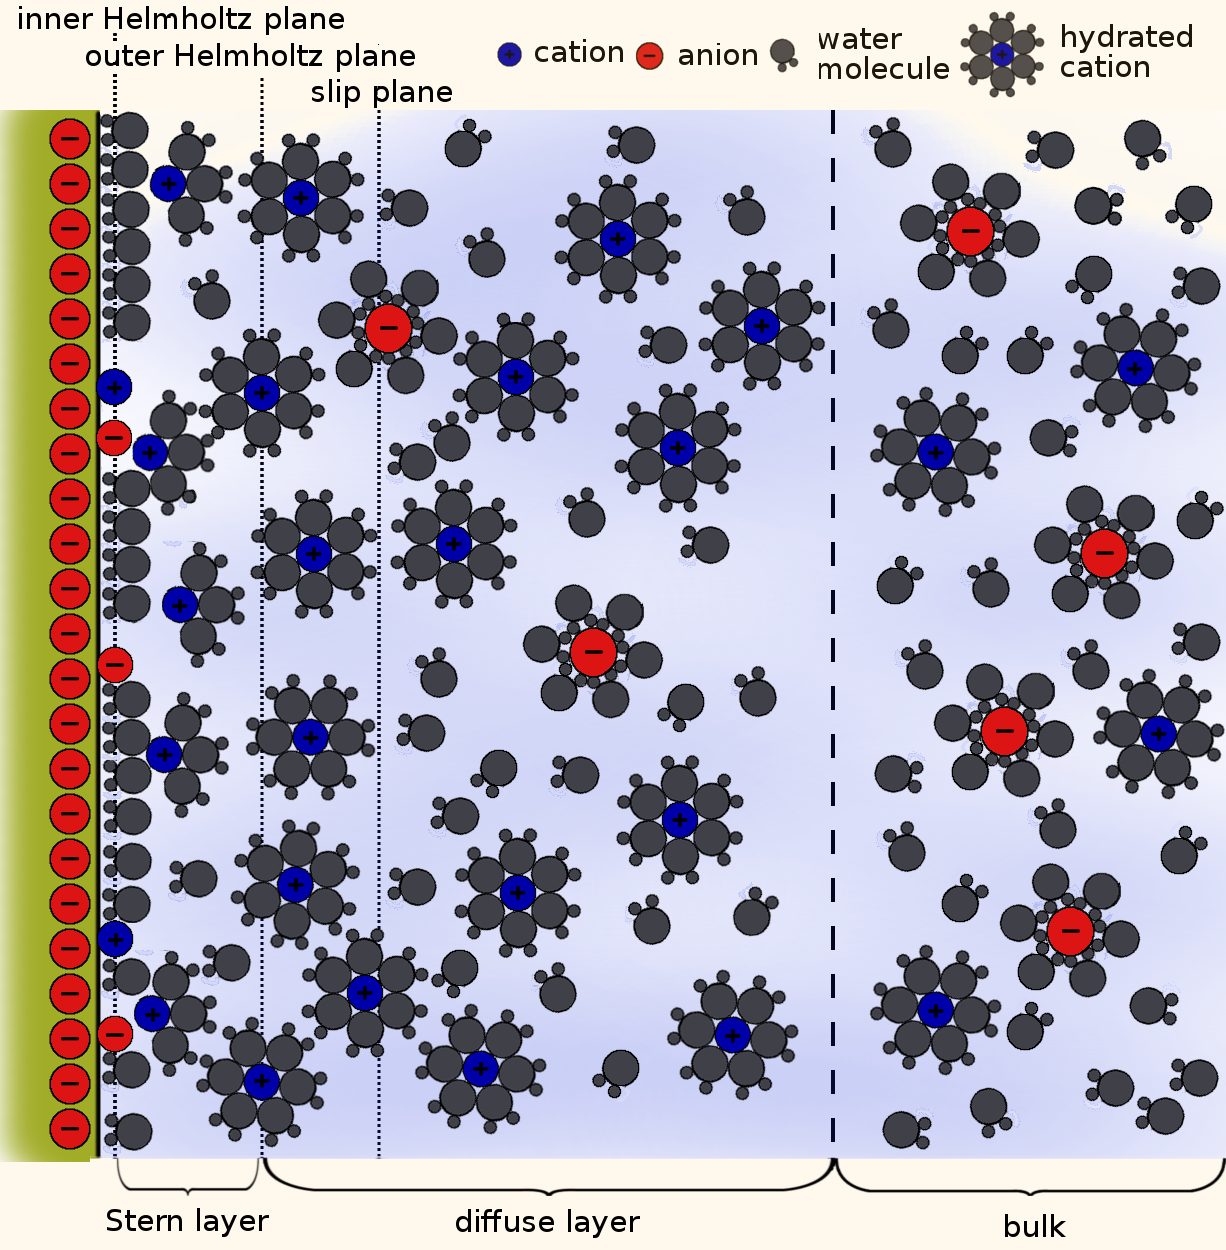
\includegraphics[width=\textwidth]{edl.png}
				\caption{Scheme of the electrical double layer under the Gouy-Chapman and Stern model. There is an abundance of counterions near the pore surface and a reduced number of coions. At the bulk both ion species' concentrations are equal.}
				
				 \label{fig:edl}
			\end{figure}
			
			Because the ion solution is conductive, mobile ions outside the Stern layer will redistribute themselves near the charged surface to counter or `screen' its $\zeta-$potential. This screening layer is known as the Debye layer, and is characterized by an enriched number of counterions (ions of opposite charge polarity to the wall) and a depleted number of coions. As we will see, the electrical double layer has a characteristic length scale known as the Debye length $\lambda_{D}$, which ranges from $0.1-10$ nm for most solution concentrations. Figure \ref{fig:edl} gives a view of the electrical double layer under the combined Gouy-Chapman and Stern models. 

			
			\begin{figure}
				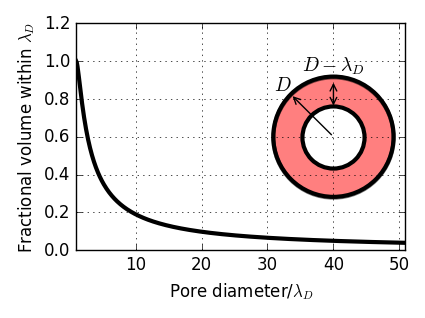
\includegraphics{fractioninsideedl.png}
				\caption{Plot of fraction of volume in a nanopore that is within the EDL versus pore diameter. The plot reveals a large super linear increase of total solution within the EDL as diameter decreases, starting at approximately $D\approx 10\lambda_{D}$.}
				
				\label{fig:fractioninsideedl}
			\end{figure}
			
			Nanopore's interesting behavior emerges when a non-negligible amount of the total volume is within a distance of $\lambda_{D}$ of the pore wall. Assuming $\lambda_{D}=1$, figure \ref{fig:fractioninsideedl} shows the fractional area of pore contained within $\lambda_{D}$ of the pore wall as a function of the pore diameter $D$. 
			
			
			
			For pores with diameter $D\gtrsim10\lambda_{D}$, the total volume within the electrical double layer is negligible; however, below approximately $10\lambda_{D}$ the total volume within the EDL quickly increases. This explains why the `nano' prefix in nanopore is important; as we approach the scale of the EDL, the structure of the solution very quickly changes, in a non-linear fashion, within the vicinity of a few nm of the pore wall.
			
			
			
			In order to derive the appearance of the EDL, we consider the equations governing the distribution of ions in solution. In the solution, the ion species $i$ have an electrostatic potential energy $U_{i}=z_{i}e\phi$, and have the following distribution in accordance with Boltzmann statistics
			
			
			
			\begin{equation} \label{eq:boltzmann}
				c_{i}=c_{0,i}\mathrm{e}^{-\frac{z_{i}e\phi}{k_{B}T}}.				
			\end{equation}
			
			The electric potential itself is given by the Poisson equation
			
			\begin{equation} \label{eq:poisson}
				\begin{split}
					\matr{\nabla}^{2}\phi & = -\frac{\rho}{\epsilon} \\
					\matr{\nabla}^{2}\phi & = -\frac{1}{\epsilon}\sum_{i}z_{i}ec_{i}\left(y\right).
				\end{split}
			\end{equation}
			
			Plugging the concentrations given by the Boltzmann equation into the Poisson equation, we arrive at the Poisson-Boltzmann equation
			
			\begin{equation} \label{eq:pb}
				\matr{\nabla}^{2}\phi=-\frac{1}{\epsilon}\sum_{i}z_{i}ec_{0,i}\mathrm{e}^{-\frac{z_{i}e\phi}{k_{B}T}}.
			\end{equation}
			
			The Poisson-Boltzmann equation \ref{eq:pb} is a second order non-linear differential equation for the electrostatic potential $\phi$; after solving for $\phi$, it can be plugged back into the Poisson equation \ref{eq:poisson} to obtain the ion concentrations $c_{i}$. The Poisson-Boltzmann equation is generally solved numerically, but analytic solutions exist for simplified assumptions about the geometry and magnitude of the electrostatic potential in the solution. 
			
			Consider a planar surface with unit normal pointing in the $\hat{y}-$ direction and uniform surface charge density $\sigma$ immersed in a solution of water and symmetric ions with molar concentration $c_{\pm}$, valency $z_{\pm}=z$, and identical diffusion coefficients $D_{i}$; this ion configuration is a close approximation of a KCl electrolyte solution, a common-used electrolyte in nanopore experiments due to the near-perfect symmetry of the ions. The ions have electrostatic potential energy given by $U_{i}=z_{i}\mathrm{e}\phi\left(y\right)$ where the electric potential $\phi$ is only a function of distance from the wall due to the system's symmetry. Under these assumptions, the Poisson-Boltzmann equation becomes
			
			\[ \frac{d^{2}\phi}{dy^{2}}=-\frac{zec_{0}}{\epsilon}. \]
			
			Though the solution can be solved analytically, a simple solution is obtained when we linearize the right hand side of the equation under the assumption $zec_{0}\ll k_{B}T$ and apply the correct boundary conditions, an approximation known as the Debye-H\u ckel approximation. The solution is
			
			\begin{equation} \label{eq:pb1d}
				\begin{split}
					\phi &= \phi_{0}\mathrm{e}^{-\frac{y}{\lambda_{D}}} \\
					c_{i} &= c_{i,0}\mathrm{e}^{-\frac{z_{i}e\phi_{0}}{k_{B}T}\mathrm{e}^{-y/\lambda_{D}}} \\
					\lambda_{D} &= \sqrt{\frac{\epsilon k_{B}T}{2c_{0}}}z,
				\end{split}				
			\end{equation}
			
			\begin{figure}
				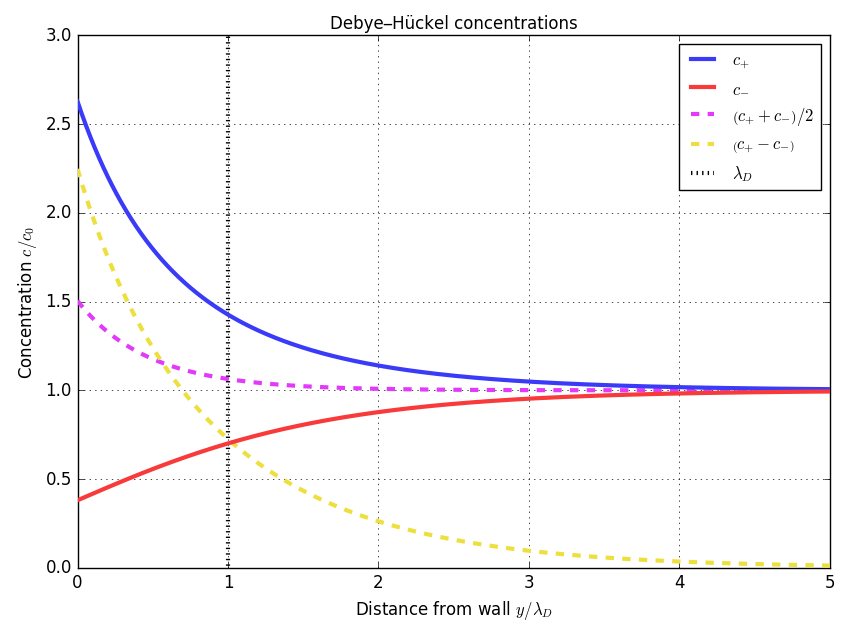
\includegraphics[width=\textwidth]{EDL_Charge_Distribution.png}
				\caption{\textbf{Ion concentrations adjacent to a negatively charged surface according to the Debye-Huckel theory.} The plot reveals that the counterion concentration (blue) is enhanced near the wall, and decays approximately exponentially as distance from the wall increases. Oppositely, coions (red) are diminished near the wall, and rise to their bulk value with distance from the wall. The \textit{total} ion concentration at the pore surface is slightly higher than the total ion concentration in the bulk. The space charge density $\rho_{E}\propto\left[c_{+}\left(y\right)-c_{-}\left(y\right)\right]$ is non-zero near the wall, and decays to zero in the bulk.}
				\label{fig:EDLChargeDistribution}
			\end{figure}

			
			where we introduced a new parameter, the Debye length $\lambda_{D}$. The solution to the 1-D lineared Poisson-Boltzmann equation reveals that the electrostatic potential exponentially approaches 0 from the wall, that the counterion species are enriched at the surface and diminish towards the bulk, and the coions are diminished at the surface, but recover their concentration towards the bulk. The Debye length is perhaps the most useful parameter in nanopore systems since it gives a characteristic length scale for the region within the pore wall that departs from its bulk, ordinary behavior. The Debye length increases with dilute ion concentrations and decreases as the ion concentration is increased, and is typically somewhere in the range of $0.1-10$ nm for common solution preparations. Note that although we discussed the electrical double layer here in the context of a pore surface, nearly every body immersed in solution will have some surface charge and therefore its own electrical double layer. The electrical double layers of free-bodies i.e.~particles are integral in explaining their motion in applied electrical fields, also known as electrophoresis. 
			
			The importance of the EDL in bestowing nanopores with their novel conductance properties cannot be overstated, and accordingly there are many phenomenon that nanopores that exhibit that are a direct consequence of the present of the EDL. In the next few sections we will review some of these phenomena.
			
			
		\subsection{Electroosmosis}
			
			Ions migrate in externally applied electric fields, and ions of opposite polarity travel in opposite directions. When ions move, they tend to drag fluid along with them. In the bulk, this fact results in no net motion of fluid because for every anion that drags fluid towards the cathode, there is a cation that drags fluid towards the anode, and the two motions cancel each other out so that there is no net motion of fluid. However, as we've just learned there \textit{is} a net concentration of one ion polarity in the EDL, so we expect that an electric field applied parallel to a charged surface will induce motion of the fluid. This intuition turns out to be correct, and the effect is known as electroosmosis. Interestingly, although the effect originates due to the presence of the $\sim \SI{1}{nm}-$thick EDL, the induced fluid flow propogates well into the bulk, and electroosmosis is observable in micro- and even milli-sized systems. This result, while surprising, is due to the simple viscous coupling of the fluid at the EDL surface to the rest of the fluid.
			
			Because electroosmosis induces a general fluid flow, the effect couples with the motion of all unbound actors in the system, namely the ions species and any particles suspended in the solution. In typical nanopores, convection in the electroosmotic flow tends to be less pronounced than migration in the electric field. However, some lightly charged particles for instance will only experience a small force from the electric field (electrophoresis) compared to the drag force from the fluid moving electroosmotically, and their motion is therefore determined primarily by electroosmosis. For the case of ions, usually the electroosmotic convective velocity adds or subtracts only a small offset to their net total motion, which remains dominated by electrophoresis. However, recently it was shown that some types of channels exhibit frictionless flow of water, and in these cases the electroosmotic velocities can become very large. In these channels it is actually expected that electroosmotic offers a large, if not dominant contribution to the motion of ions in the system. One example of these special types of pores, carbon nanotube pores, will be discussed later in this dissertation.
			
			To understand electroosmosis, we look to the Navier-Stokes equations which describe the motion of fluids, and the Poisson-Boltzmann equation which yields the distribution of ions in the vicinity of the EDL. As an example, consider again an infinite charged plane with unit normal pointing in the $\hat{y}-$ direction, but this time with a constant electric field $\vec{E}$ applied parallel to its surface. The Navier-Stokes equation (eq \ref{eq:ns}) simplifies greatly in this case, and simply becomes
			
			\[ 0 = \eta\frac{\partial^{2}u}{\partial y^{2}}+\left[c_{+}\left(y\right)-c_{-}\left(y\right)\right]zeE_{ext}. \]
			
			The equation shows that there is a momentum flux source term from the electric field acting on the charged solution in the EDL, which is proportional to the net charge in the solution (proportional to $c_{+}-c_{-}$) times the electric field $\vec{E}$. The other term that balances the driving force is due to viscous forces between neighboring layers that have different $y-$ velocities $u$, i.e. due to velocity gradients perpendicular to the wall. In order to solve this equation, we can replace the charge density $\rho_{E}=ze\left(c_{+}-c_{-}\right)$ with the Laplacian of the scalar potential $\phi$, integrate twice, and apply the correct boundary conditions, that the velocity at the pore wall is 0 (the so-called `non-slip' boundary condition) and that the velocity gradients are 0 infinitely far from the wall.  Performing these steps, we find the fluid velocity equals 
			
			\[ u=\frac{\epsilon E_{ext}}{\eta}\left(\phi-\zeta\right), \]
			
			where $\phi_{0}$ is the electric potential immediately outside the surface charges on the pore wall. Interestingly, according to this equation the fluid velocity is proportional to the local electric potential in the screening layer, which is determined by solving the Poisson-Boltzmann equation (Eq. \ref{eq:pb}). Under the Debye-H\u ckel approximation of small surface potentials, the fluid velocity is zero at the walls, and exponentially approaches its bulk value as distance from the wall increases. This type of fluid flow profile is known as `plug flow', since the velocity is approximately constant everywhere except in the thin EDL where there are sharp velocity gradients. Since the potential in the bulk is equal to $\phi=0$, we find the bulk velocity to be equal to 
			
			\begin{equation} \label{eq:hs}
				\begin{split}
					u &= -\frac{\epsilon\zeta}{\eta}E_{ext} \\
					u &= \mu_{EO}E_{ext},
				\end{split}
			\end{equation}
			
			

			
			a result known as the Helmholtz-Smoluchowski equation. The parameter $\mu_{EO}\equiv-\frac{\epsilon\zeta}{\eta}$ introduced is known as the electroosmotic mobility, and is the proportionality constant between the applied electrical field and the resulting fluid velocity. Typical values of the mobility are $\mu_{EO}=10^{-8} \left[m^{2}/V s\right]$, which for an electric field of $\SI{1}{V/\mu m^{2}}$ yields a fluid velocity of approximately $\SI{1}{cm/s}$. 
			
			\begin{figure}
				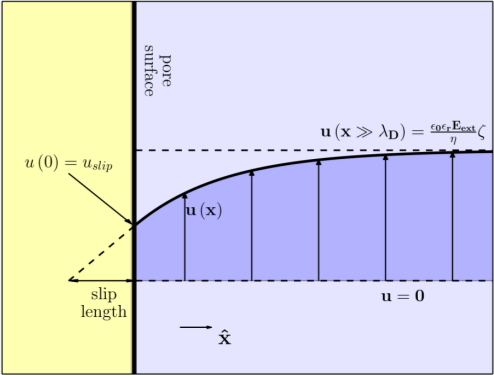
\includegraphics[width=.5\textwidth]{electroosmosis.png}
				\caption{\textbf{Plot of electroosmotic flow along an infinite plane with finite slip length}. A net ion charge at the surface experiences a force in an electric field which drags fluid along with it. The force is only present in the electrical double layer, which viscously couples to the rest of the fluid. This fluid flow profile is known as plug flow, and extends far beyond the EDL where it originates.}
				\label{fig:electroosmosis}
			\end{figure}
			
			Figure \ref{fig:electroosmosis} shows the fluid flow profile in a pore with a finite slip length $u_{\mathrm{slip}}$; however, it must be noted that in the vast majority of experimental systems, $u_{\mathrm{slip}}=0$.
			
			It is possible to experimentally observe the fluid flow velocity, for instance by tracking the motion of small particles that move in the fluid flow, and therefore Eq. \ref{eq:hs} provides a means for directly measuring the $\zeta-$potential.
			
		\subsection{Surface conductance and conductance saturation}
		
			\begin{figure} 
				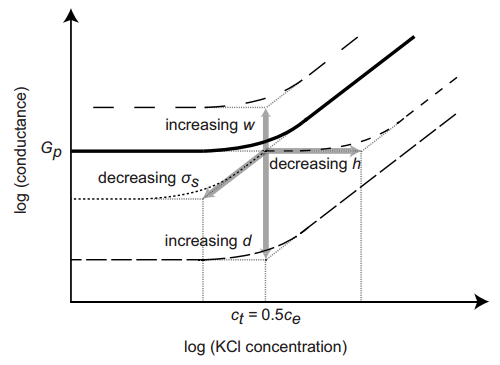
\includegraphics[width=0.5\textwidth]{Schoch2008_conductance}
				\caption{Reprinted (abstract/excerpt/figure) with permission from [(FULL REFERENCE CITATION) as follows: Author's Names, APS Journal Title, Volume Number, Page Number and Year of Publication.] Copyright (YEAR) by the American Physical Society.}
				\label{fig:Schoch2008conductance}
			\end{figure}
		
			Ignoring electrical double layer effects, the conductance of an ion channel is proportional to the ion concentration in the solution; doubling the ion concentration exactly doubles the measured current. However, the presence of the electrical double layer breaks this perfect linear conductance relationship for two reasons. First, the integrated \textit{excess} ion count $\int_{0}^{EDL}=\left[\left(c_{+}+c_{-}\right)-2c_{0}\right]dy$ in the EDL layer is not guaranteed to be the same as the total ion concentration in the bulk; in fact, in most cases it is slightly higher, meaning the electrophoretic current in the EDL is slightly higher than in the bulk. Another important contribution to the measured current is the current from convection due to electroosmosis; because there is a net charge density in the fluid, electroosmosis will create a measurable ion current! In total, there are three terms that contribute to the total current measured in a channel, migration of ions in the bulk, migration of the integrated ion \textit{excess} in the EDL, and net convection of charge in the EDL due to electroosmosis. Without applying any equations, we can use what we learned about the EDL and some general logic to reason about what the current behavior should be in the limiting cases of very large ion concentration and very small ion concentration. The equation for the Debye-length is $\lambda_{D}\propto c_{0}^{-1/2}$; for very large ion concentration, the EDL should be negligible and therefore neither the effects of electroosmosis nor electrophoretic ion excess should be significant. At the other end of the scale, in the limit of nearly zero ions in the bulk we still must have charge neutrality in the pore, meaning a finite concentration of ions despite the bulk concentration being zero. In this case, the EDL fills the entire pore and the result is that the conductance is entirely due to the integrated excess and convective terms. This finite conductance at zero concentration is known as the \textit{saturation current}. Therefore, as we increase the length of the EDL we expect the conductance discrepancy, the difference in bulk conductance versus conductance due to the two surface effects, to increase. The end result of all this is that the conductance is a non-linear function of ion concentration at sufficiently low ion concentration; removing ions past some point does not further reduce the conductance of the channel! Consider a nanopore immersed in solution of two symmetric ions denoted $+$ and $-$ (symmetric means their mobilities, valencies, and bulk concentrations are equal) with electrophoretic mobility $\mu_{EP}$ and electroosmotic mobility $\mu_{EP}$. The following expression breaks down the total measured current into the three components described above:
		
			
			\begin{equation} \label{eq:totalconductance}
				\begin{split}
					I &= I_{\mathrm{bulk}}+I_{\mathrm{excess}}+I_{\mathrm{EO}} \\
					I &= \int 2c_{0}\mu_{EP}EezdA + \int\left[c_{+}\left(z\right)+c_{-}\left(z\right)-2c_{0}\right]\mu_{EP}EezdA + \int\left[c_{+}\left(z\right)-c_{-}\left(z\right)\right]u_{\mathrm{EO}}\left(z\right)ezdA.
				\end{split}
			\end{equation}
			
			Figure \ref{fig:Schoch2008conductance} shows a plot of the conductance versus solution concentration for a nanopore; the plot reveals a saturation at low solution concentration as expected from the preceding arguments. The saturation current is equal to the surface conductance term in the above equation.
			
		\subsection{Ion selectivity}
			A phenomenon related to surface conductance is \textit{ion selectivity}. Since the EDL has a higher concentration of counterions rather than coions, the total flux of ions through the pore is slightly skewed towards counterions. The ion selectivity is defined as
			
			\begin{equation} \label{eq:selectivity}
				S=\frac{|I_{+}-I_{-}|}{I}.				
			\end{equation}
			
		
		\subsection{Ionic current rectification}
			An ion channel is said to be rectifying if its conductance for one voltage polarity is greater than the opposite voltage polarity. The presence of an EDL alone cannot account for this, since the system has symmetry with respect to switching the electrodes, and therefore no rectification will occur. However, by introducing asymmetry into a system, along with having the pore be partially ion selective, we can create rectifying pores. There are many ways to create asymmetric nanopores, but two obvious solutions are geometry and surface charge pattern based.
			
			If the shape of a nanopore is asymmetric, for instance as in a cone, the ionic current will be rectified. A simple explanation for this is that at the tip-side of the pore (in the case of conical nanopores), there will be an excess of counterions in the vicinity of the entrance EDL, while the other side will more closely resemble the bulk. Because these ions are at the entrance of the pore, they will more easily enter the pore than when at the other side. The result is that for one voltage polarity the ionic current is greater than at the opposite polarity.
			
			By similar reasoning, charge patterning asymmetry can also lead to rectification. By placing two charges of opposite polarity adjacent to one another inside the pore, for one voltage polarity a depletion zone is created in analogy with the depletion zone formed between the n- and p-doped regions in a semiconductor diode. The ionic current is rectified, and because the diode junction so severely limits the ionic current under one voltage polarity, the device is said to be equivalent to an ionic diode.\cite{Vlassiouk2007}
			
			\begin{figure}
				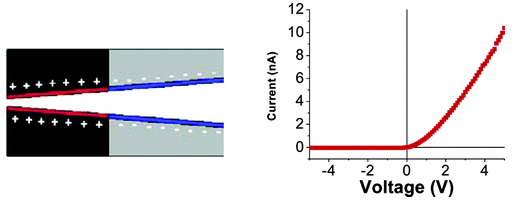
\includegraphics[width=.5\textwidth]{Vlassiouk2007_conicaldiode}
				\caption{\textbf{An ionic diode formed in a conical nanopore with bipolar surface charge patterning.} The region between negative and positive charges is the depletion zone, and provides a large resistance to ion flow through the pore for one voltage polarity. Reprinted with permission from \bibentry{Vlassiouk2007}. Copyright 2007 American Chemical Society.}
				\label{fig:Vlassiouk2007conicaldiode}
			\end{figure}
			
			Figure \ref{fig:Vlassiouk2007conicaldiode} shows a conical nanopore with a bipolar charge distribution. The combination of the geometrical and charge asymmetry gives the pore a very large rectification value, and the near-zero current for one polarity of voltage is enough to consider the pore a diode.

			
			


			
			
		
			
			
		
			
			

			
			
		\subsubsection{Particle electrophoresis}
			
			Electrophoresis is the transport of a charged particle in the presence of an electric field. The effect of electrophoresis can be derived much in the way electroosmosis was derived, but instead of considering the fluid flow velocity at the surface of the particle to be zero, we set it equal to the electrophoretic velocity. For particles with thin electrical double layers (Debye-H\u ckel approximation) and laminar flow (Stoke's flow), the particle velocity is
			
			\begin{equation} \label{eq:electrophoresis}
				\begin{split}
					\vec{u} &= \frac{\epsilon\vec{E}_{0}}{\eta}\phi_{0} \\
					\vec{u} &= \mu_{\mathrm{EP}}=\frac{\epsilon\phi_{0}}{\eta}.
				\end{split}
			\end{equation}
			
			In equation \ref{eq:electrophoresis}, we've again introduced a proportionality factor between the applied electric field $E_{0}$ and the induced velocity $\vec{u}$; this factor is known as the electrophoretic mobility. However, these equations are derived under the assumption that the applied electric field does not perturb the distribution of ions in the electrical double layer, which is only true for small surface potentials. If this assumption is invalid, additional effects related to the redistribution of ions must be taken into account; the net effect is a retarding force on the particle that slows its velocity.
			
			Electrophoresis is an important effect in many applications involving particles. One useful application is that particle electrophoresis through a nanopore can be used to measure the zeta potential of a particle, related to its surface chemistry and chemical adsorption. An electric field is applied across a nanopore which is immersed in electrolyte solution containing ions and charged particles. Particles travel through the pore under electrophoresis, and the dwell time can be recorded using resistive pulse sensing or optical techniques. If the geometry of the pore is known, the dwell time can be related with the particle velocity, and the electric field strength can be determined as well. In this case, equation \ref{eq:electrophoresis} can be solved for the surface potential $\phi_{0}$, which is the same as its zeta-potential.
			
		\subsubsection{Particle electrophoresis + electroosmosis}
			Transport of particles is in general a superposition of electrophoretic and electroosmotic effects. Combining the two, the velocity of a charged particle translocating through a charged pore is 
			
			\begin{equation} \label{eq:particlevelocity}
				\begin{split}
					v=\left(\mu_{EP}+\mu_{EO}\right)E, \\
					v=\frac{\epsilon}{\eta}\left(\zeta_{\mathrm{particle}}-\zeta_{\mathrm{pore}}\right)E
				\end{split}
			\end{equation}
			
			In general the net velocity can be positive, negative, or zero depending on the relative sizes and signs of the electrophoretic mobility.



			

			
			
			

			
			
			
			

			
			


			
	





%%% Local Variables: ***
%%% mode: latex ***
%%% TeX-master: "thesis.tex" ***
%%% End: ***

% ... and so on

% These commands fix an odd problem in which the bibliography line
% of the Table of Contents shows the wrong page number.
\clearpage
\phantomsection

% "References should be formatted in style most common in discipline",
% abbrv is only a suggestion.

\bibliographystyle{abbrv}
\bibliography{../../LaTeX/references/references}

% The Thesis Manual says not to include appendix figures and tables in
% the List of Figures and Tables, respectively, so these commands from
% the caption package turn it off from this point onwards. If needed,
% it can be re-enabled later (using list=yes argument).
\captionsetup[figure]{list=no}
\captionsetup[table]{list=no}

% If you have an appendix, it should come after the references.
% The original template (from Trevor) had a custom \appendix command,
% but I found it to break figure/table counters. I'm not sure how
% reliable my fix is, so I ended up reverting back to the standard
% latex version, and renaming the custom command to \myappendix.  You
% can try both and see how things work out:
% 1) Call \appendix once, and then make each appendix a \chapter
% 2) Call \myappendix once, and then make each appendix a \section.

\appendix
\chapter{Appendix Title}


\section{Lorem Ipsum}




%%% Local Variables: ***
%%% mode: latex ***
%%% TeX-master: "thesis.tex" ***
%%% End: ***


\end{document}
